%%%%%%%%%%%%%%%%%%%%%%%%%%%%%%%%%%%%%%%%%%%%%%%%%%%%%%%%
%%
\chapter{Summary of changes (AT-4)}
\label{ch:changelog}
%%
%%%%%%%%%%%%%%%%%%%%%%%%%%%%%%%%%%%%%%%%%%%%%%%%%%%%%%%%

Below we describe breifly the main differences from AT-4 build.

%%%%%%%%%%%%%%%%%%%%%%%%%%%%%%%%%%%%%%%%%%%%%%%%%%%%%%%%
%%
\section{General}
%%
%%%%%%%%%%%%%%%%%%%%%%%%%%%%%%%%%%%%%%%%%%%%%%%%%%%%%%%%
\begin{itemize}

\item all recipes main body of code is now in a \defineprogram{\progMAIN} function and this function is called in \defineprogram{\MAIN} part of the code (the part that executes at run time). This allows recipes to be called as functions as well as being called as a standalone code or from the command line. i.e. for \calDARK:
	\begin{pythonbox}
	import cal_DARK_spirou
	    
	files = ['dark_dark02d406.fits']
	night_name = '20170710'
	cal_DARK_spirou.main(night_name=night_name, files=files)
	\end{pythonbox}
	will run the exact same procedure as:
	\begin{bashbox}
	cal_DARK_spirou.py 201707 dark_dark02d406.fits
	\end{bashbox}

\item \WLOG function overhal (now in \spirouLog.logger()) but aliased in most codes back to \WLOG. This means one can use the same functionality as before:
	\begin{pythonbox}
	WLOG("warning", "program", "message")
	\end{pythonbox}
	In addition:
	\begin{itemize}
	\item when "error" is called an automatic exit routine is run (therefore there is no need for sys.exit after a \WLOG("error", "", "") call).

	\item log printed to standard output (console) can be coloured (see \definevariable{text:colouredlevels}{coloured levels}) this functionality can be switched off and on easily, but with it on errors are coloured red and warning coloured yellow (greatly increases usability).

	\end{itemize}
\item execution of pythonstartup codes removed and replaced with setup functions (easier to manage, all variables loaded into parameter dictionary (\ParamDict) with their definition location defined (source).

\item loading of many variables into python memory replaced with call to need dictionary object (parameter dictionary). Parameter dictionary is a custom dictionary object that as well as storing key and value pairs also can set a source for each key in the dictionary (hence the developer will always know where a variable was defined, if used correctly)

\item All hard coded constants removed from running code and moved to configuration files, all variables have been described, noted their new definition locations and where they are used in the recipes and codes (see Section \ref{ch:variables}). This has allowed (and will allow) variables to either be public (i.e. in a location easily accessible by the user) or to be private (in files stored within the module). We can make many specific configuration files or a few, depending on which we deem best.

\item Custom exception: \ConfigError and \definevariable{ch:rules:drs_specific:config_error}{ConfigException} - designed specifically to be used with the \WLOG function 

\item moved core functions used in multiple recipes to sub-modules

\item all plotting taken out of main codes (call to specific sub-module)

\item calibration database slightly reworked:

\begin{itemize}
	\item Lines can now be commented (i.e. by starting a line with a \#)
	\item Blank lines are now ignored (helps for usability)
	\item Two options for selecting sources with multiple keys the same (i.e. two or more with key ``dark'') this is set with \definevariable{text:calib_db_match}{calib\_db\_match} options are:

	\begin{itemize}
		\item `older' (same as AT4 V48 where only calibDB files older than the unix time of `fitsfilename' is selected and the one closest to the unix time of `fitsfilename' is used).
		\item `closest' - selects the calibDB file that is closest in time to the unix tome of `fitsfilename'
	\end{itemize}
	\begin{note}
	If two calibDB files with the same key have the same unix time, the one lower in the list is used.
	\end{note}

	\item there is also a test that the human readable date and unix date are the same (error is raised if they are different)
	\DevNote{This may be taken out, but it seems that the unix time and human reabable time should be the same.}

\end{itemize}

\end{itemize}


%%%%%%%%%%%%%%%%%%%%%%%%%%%%%%%%%%%%%%%%%%%%%%%%%%%%%%%%
%%
\section{The Recipes}
\label{ch:changelog:At4:recipes}
%%
%%%%%%%%%%%%%%%%%%%%%%%%%%%%%%%%%%%%%%%%%%%%%%%%%%%%%%%%


%%%%%%%%%%%%%%%%%%%%%%%%%%%%%%%%%%%%%%%%%%%%%%%%%%%%%%%%
%%
\subsection{The cal\_DARK\_spirou recipe}
\label{ch:changelog:At4:cal_DARK_spirou}
%%
%%%%%%%%%%%%%%%%%%%%%%%%%%%%%%%%%%%%%%%%%%%%%%%%%%%%%%%%

\begin{itemize}

\item dark measurement moved to function \spirouImage.MeasureDark (for clarity). This is, in part, due to the repetition of code for ``Whole det'', ``Blue part'' and ``Red part''.

\item all plotting moved to internal functions (for clarity)
	\begin{itemize}
    \item \spirouPlot.darkplot\_image\_and\_regions for the image/region plot
    \item \spirouPlot.darkplot\_datacut for the DARK cutlimit plot
    \item \spirouPlot.darkplot\_histograms for the histogram plots 
    \end{itemize}

\item histogram plot updated, original plot plotted bin centers as a smooth peak, simple modification to make sure histogram bars are present
    
\item writing of data is sped up by caching all HEADER keys and writing to file once with the write of the data.

\item speed up
	\begin{itemize}
	\item AT-4 v44: 4.881 seconds
	\item py3: 1.890 seconds
	\end{itemize}

\end{itemize}

%%%%%%%%%%%%%%%%%%%%%%%%%%%%%%%%%%%%%%%%%%%%%%%%%%%%%%%%
%%
\subsection{The cal\_loc\_RAW\_spirou recipe}
\label{ch:changelog:At4:cal_loc_RAW_spirou}
%%
%%%%%%%%%%%%%%%%%%%%%%%%%%%%%%%%%%%%%%%%%%%%%%%%%%%%%%%%

\begin{itemize}

\item added function to convert from ADU/s to electrons \spirouImage.ConvertToE
    
\item added function to flip image \spirouImage.FlipImage

\item smoothed image (by a box) is now in a function (creates order\_profile)
	\begin{itemize}
	\item added different way to calculate order\_profile - currently set to 'manual' be default
	\item \spirouLOCOR.BoxSmoothedImage 
	\item Instead of manually working out the mean for each box you convolve the weighted image with a tophat function and the weights with a topcat function and then divide the two.
	\item This gives approximately the same result (with small deviations due to the FT of a topcat function not being perfect).
	\item The function can be turned back to the original manual mode by using `mode='manual'' but is slower (by a factor of $\sim\times$8)
	\end{itemize}

\item added storage dictionary to store (and pass around) all variables created `loc' - a Parameter dictionary (thus source can be set for all variables to keep track of them)

\item added function to measure background and get central pixel positions \spirouLOCOR.MeasureBkgrdGetCentPixs

\item debug plot added to plot the minimum of `ycc' and `ic\_locseuil' \spirouPlot.sPlt.debug\_locplot\_min\_ycc\_loc\_threshold

\item added function for locating central position (previously \spirouLOCOR.poscolc) - currently set to 'manual' be default
    \begin{itemize}
    \item \spirouLOCOR.LocateCentralOrderPositions
    \item  Instead of manually working out the starts and ends of each order (with while loops) convolves a mask of cvalues > threshold with a top-hat (size=3) function such that all edges are found
    \item i.e. `[False, True, True]` or `[True, True, False]` give a different value than `[True, True, True]` or `[False, False, False]` or `[False, False, True]`
    \item i.e. the convolution gives the sum of three elements, thus selected those elements with a sum of 2 give our edges
    \item The function can be turned back to the original 'manual' mode by using `mode='manual` but is slower (by a factor of x2)
	\end{itemize}

\item debug plot added to plot the image above saturation threshold \spirouPlot.locplot\_im\_sat\_threshold
        
\item moved `ctro`,`sigo`,`ac`,`ass` etc into loc (for storage and ease of use)        
        
\item the fit across each order has been split into functions
    \begin{itemize}
	\item the initial fit is done by \spirouLOCOR.InitialOrderFit
	\item This initial fit takes in the plotting args and thus as order is fit the fit is piped on to plot via \spirouPlot.locplot\_order
	\item the sigma clipping fit is done by \spirouLOCOR.SigClipOrderFit
	\item kind is used to change between 'center' and 'fwhm' fits (thus function is reused in both cases), kind will do the tiny bits of code which are different for each fit
	\item all fit parameters are loaded into the `loc` parameter dictionary
	\end{itemize}

\item plot of order number against rms is move to \spirouPlot.locplot\_order{\hskip 0pt}\_number\_against\_rms

\item function created to add the 2Dlist (i.e. the coefficients) to hdict (the dictionary used to save keys to so that we only write to the fits file once)

\item superimposed fit on the image is pushed into a function, this is many times faster than before - due to optimisation, \spirouLOCOR.imageLocSuperimp

\item Writing of fits file cleaned up (header keywords written during data write)

\item speed up
	\begin{itemize}
	\item AT-4 v44: 5.697 seconds
	\item py3:  2.255 seconds
    \end{itemize}

\end{itemize}

%%%%%%%%%%%%%%%%%%%%%%%%%%%%%%%%%%%%%%%%%%%%%%%%%%%%%%%%
%%
\subsection{The cal\_SLIT\_spirou recipe}
\label{ch:changelog:At4:cal_SLIT_spirou}
%%
%%%%%%%%%%%%%%%%%%%%%%%%%%%%%%%%%%%%%%%%%%%%%%%%%%%%%%%%

\begin{itemize}
\item added storage dictionary to store (and pass around) all variables created `loc` - a Parameter dictionary (thus source can be set for all variables to keep track of them)

\item Retrieval of coefficients from `\_loco\_` file moved to \spirouLOCOR.GetCoeffs

\item Tilt finding is moved to function \spirouImage.GetTilt

\item Fitting the tilt is moved to function \spirouImage.FitTilt

\item selected order plot moved to \spirouPlot.slit\_sorder\_plot

\item slit tilt angle and fit plot moved to \spirouPlot.slit\_tilt\_angle\_and\_fit\_plot

\item Writing of fits file cleaned up (header keywords written during data write)

\item speed up
	\begin{itemize}
	\item AT-4 v44: 11.071 seconds
	\item py3: 4.386 seconds
    \end{itemize}

\end{itemize}

%%%%%%%%%%%%%%%%%%%%%%%%%%%%%%%%%%%%%%%%%%%%%%%%%%%%%%%%
%%
\subsection{The cal\_FF\_RAW\_spirou recipe}
\label{ch:changelog:At4:cal_FF_RAW_spirou}
%%
%%%%%%%%%%%%%%%%%%%%%%%%%%%%%%%%%%%%%%%%%%%%%%%%%%%%%%%%

\begin{itemize}
\item added function to replace measure\_bkgr\_FF, but incomplete (not currently used) would need to convert interpol.c to python (spline fitting)

\item added storage dictionary to store (and pass around) all variables created `loc` - a Parameter dictionary (thus source can be set for all variables to keep track of them)

\item Created function to read TILT file from calibDB (replaces `readkeyloco`)
	\begin{itemize}
    \item \spirouImage.ReadTiltFile
    \item takes in header dictionary from `fitsfilename` in order to avoid re-opening FITS rec (acqutime used in calibDB to get max\_time of calibDB entry) 
    \end{itemize}
\item Created function to read order profile (replaces `read\_data\_raw` + pre-amble)
	\begin{itemize}
	\item \spirouImage.ReadOrderProfile
	\item takes in header dictionary from `fitsfilename` in order to avoid re-opening FITS rec (acqutime used in calibDB to get max\_time of calibDB entry) 
    \end{itemize}
\item Used \spirouLOCOR.GetCoeffs to get the coefficients from file

\item Created merge coefficients function to perform AB coefficient merge \spirouLOCOR.MergeCoefficients
    
\item Updated extraction function \spirouEXTOR.ExtracTiltWeightOrder2 - much faster as takes many of the calculations outside the pixel loop
	\begin{itemize}
	\item i.e. calculating the pixel contribution due to tilt in array `ww`
	\item `ww` is constant for an order, thus doesn't need to be worked out for each pixel in one order, just the multiplication between ww and the image
	\item up to 8 times faster with these improvements
    \end{itemize}
\item `e2ds`, `SNR`, `RMS`, `blaze` and `flat` are stored in `loc` parameter dictionary

\item Plotting code moved to \spirouPlot functions

\item Writing of fits file cleaned up (header keywords written during data write)

\item QC (max\_signal $>$ qc\_max\_signal $\times$ nbframes) moved to end, however in old code it is not used as a failure criteria so also not used to fail in new code

\item speed up
	\begin{itemize}
	\item AT-4 v44: 25.962 seconds
	\item py3: 4.675 seconds
    \end{itemize}

\end{itemize}

%%%%%%%%%%%%%%%%%%%%%%%%%%%%%%%%%%%%%%%%%%%%%%%%%%%%%%%%
%%
\subsection{The cal\_extract\_RAW\_spirou recipes}
\label{ch:changelog:At4:cal_extract_RAW_spirou}
%%
%%%%%%%%%%%%%%%%%%%%%%%%%%%%%%%%%%%%%%%%%%%%%%%%%%%%%%%%

\begin{itemize}
\item Merged \calextractRAWAB, \calextractRAWC and \calextractRAWALL can still access \calextractRAWAB, \calextractRAWC and \calextractRAWALL but instead of being modified copies of the code they are just wrappers for \calextractRAW (i.e. they forward the fiber type)

\item added storage dictionary to store (and pass around) all variables created `loc` - a Parameter dictionary (thus source can be set for all variables to keep track of them)

\item Created function to read TILT file from calibDB (replaces `readkeyloco`)
    \begin{itemize}
	\item \spirouImage.ReadTiltFile
	\item takes in header dictionary from `fitsfilename` in order to avoid re-opening FITS rec (acqutime used in calibDB to get max\_time of calibDB entry) 
    \end{itemize}

\item Created function to read WAVE file from calibDB (replaces `read\_data\_raw(`)
    \begin{itemize}
	\item \spirouImage.ReadWaveFile
	\item takes in header dictionary from `fitsfilename` in order to avoid re-opening FITS rec (acqutime used in calibDB to get max\_time of calibDB entry) 
    \end{itemize}

\item Used \spirouLOCOR.GetCoeffs to get the coefficients from file

\item Created function to read order profile (replaces `read\_data\_raw` + pre-amble)
    \begin{itemize}
	\item \spirouImage.ReadOrderProfile
	\item takes in header dictionary from `fitsfilename` in order to avoid re-opening FITS rec (acqutime used in calibDB to get max\_time of calibDB entry) 
    \end{itemize}

\item Created merge coefficients function to perform AB coefficient merge \spirouLOCOR.MergeCoefficients

\item New structures above replace the need for specific fiber sections ('AB', 'C', 'A', 'B') (In \calextractRAWALL and individual setups for \calextractRAWAB and \calextractRAWC)

\item all extraction functions passed into \spirouEXTOR to wrapper functions (\spirouEXTOR.ExtractOrder, \spirouEXTOR.ExtractTiltOrder, \spirouEXTOR.ExtractTiltWeightOrder and \spirouEXTOR.ExtractWeightOrder) these are then run into \spirouEXTOR.ExtractionWrapper and processed accordingly

\item Added a timing string (to record timings of all extraction processes) use `print(timing))` to view
    
\item `e2ds` and `SNR` stored in `loc`

\item Plotting code moved to \spirouPlot functions

\item Writing of fits file cleaned up (header keywords written during data write)

\item QC (max\_signal $>$ qc\_max\_signal $\times$ nbframes) moved to end, however in old code it is not used as a failure criteria so also not used to fail in new code

\item speed up
	\begin{itemize}
	\item AT-4 v44: 60.852
	\item py3: 8.694

	\item Extraction timing Py3:
		\begin{itemize}
		\item ExtractOrder = 0.025 s
		\item ExtractTiltOrder = 0.060 s
		\item ExtractTiltWeightOrder = 0.141 s
		\item ExtractWeightOrder = 0.070 s
         \end{itemize}

	\item Extraction timing AT-4 v46:
		\begin{itemize}
		\item ExtractOrder (Fortran) = 0.019 s
		\item ExtractOrder (Py2) = 0.085 s
		\item ExtractTiltOrder = 0.766 s
		\item ExtractTiltWeightOrder = 0.840 s
		\item ExtractWeightOrder = 0.156 s
         \end{itemize}

	\item Speed increase (Py3 over AT-4 v46)
		\begin{itemize}
		\item ExtractOrder (Py3 $\rightarrow$ Fortran) = slower    x 1.3 times slower
		\item ExtractOrder (Py3 $\rightarrow$ Py) = faster     x 3.4 times faster
		\item ExtractTiltOrder (Py3 $\rightarrow$ Py = faster     x12.9 times faster
		\item ExtractTiltWeightOrder (Py3 $\rightarrow$ Py) = faster    x6.0 times faster
		\item ExtractWeightOrder (Py3 $\rightarrow$ Py) = faster    x2.2 times faster
		\end{itemize}

	\end{itemize}

\end{itemize}


%%%%%%%%%%%%%%%%%%%%%%%%%%%%%%%%%%%%%%%%%%%%%%%%%%%%%%%%
%%
\subsection{The cal\_DRIFT\_RAW\_spirou recipe}
\label{ch:changelog:At4:cal_DRIFT_RAW_spirou}
%%
%%%%%%%%%%%%%%%%%%%%%%%%%%%%%%%%%%%%%%%%%%%%%%%%%%%%%%%%

\begin{itemize}
\item acqtime (bjdref) got from header using \spirouImage.GetAcqTime
	\begin{itemize}
	\item can be used to get both `human` readible and `unix` time (use key kind=`human` or kind=`unix)
	\end{itemize}

\item Created function to read TILT file from calibDB (replaces `readkeyloco`)
	\begin{itemize}
	\item \spirouImage.ReadTiltFile
	\item takes in header dictionary from `fitsfilename` in order to avoid re-opening FITS rec (acqutime used in calibDB to get max\_time of calibDB entry) 
	\end{itemize}

\item Created function to read WAVE file from calibDB (replaces `read\_data\_raw(`)
	\begin{itemize}
	\item \spirouImage.ReadWaveFile
	\item takes in header dictionary from `fitsfilename` in order to avoid re-opening FITS rec (acqutime used in calibDB to get max\_time of calibDB entry) 
	\end{itemize}

\item Used \spirouLOCOR.GetCoeffs to get the coefficients from file

\item Created function to read order profile (replaces `read\_data\_raw` + pre-amble)
	\begin{itemize}
	\item \spirouImage.ReadOrderProfile
	\item takes in header dictionary from `fitsfilename` in order to avoid re-opening FITS rec (acqutime used in calibDB to get max\_time of calibDB entry) 
	\end{itemize}

\item new extraction (see \calextractRAW above).

\item delta RV RMS calculation in \spirouRV.DeltaVrms2D
	\begin{itemize}
	\item where arguments are `speref` and `wave` (stored in `loc`)
	\item where keyword arguments are `sigdet`, `size` and `threshold` (stored in p)
	\end{itemize}

\item all functionality to do with listing files moved to \spirouImage{\hskip 0pt}.GetAllSimilarFiles - no need for "alphanumeric short"/"nice sort" - `np.sort(x)` does this
    
\item Renormlisation and cosmics correction in \spirouRV.ReNormCosmic2D
	\begin{itemize}
	\item where arguments are `speref` and `spe` (stored in `loc`)
	\item where keyword arguments are `cut`, `size` and `threshold` (stored in p)
	\end{itemize}

\item RV drift calculated
	\begin{itemize}
	\item \spirouRV.CalcRVdrift2D
	\item where arguments are `speref`, `spen` and `wave` (`speref` and `spen` stored in loc)
	\item where keyword arguments are `sigdet`, `size` and `threshold` (stored in p)
	\end{itemize}

\item added an option (drift\_type\_e2ds) to decide between getting drift using a weighted mean or using a median (to combine all orders)

\item `drift`, `errdrift`, `deltatime`, `mdrift`, `merrdrift` stored in loc

\item Writing of fits file cleaned up (header keywords written during data write)

\item speed up
	\begin{itemize}
	\item AT-4 v44: 22.556 s
	\item py3:  8.143 s
	\end{itemize}

\end{itemize}


%%%%%%%%%%%%%%%%%%%%%%%%%%%%%%%%%%%%%%%%%%%%%%%%%%%%%%%%
%%
\subsection{The cal\_BADPIX\_spirou recipe}
\label{ch:changelog:At4:cal_BADPIX_spirou}
%%
%%%%%%%%%%%%%%%%%%%%%%%%%%%%%%%%%%%%%%%%%%%%%%%%%%%%%%%%

\begin{itemize}
	\item loading of custom arguments moved to \spirouStartup.GetCustomFromRuntime

	\item loading of files moved to \spirouImage.ReadImage

	\item normalising flat and median of flat moved to \spirouImage.NormMedianFlat

	\item locating bad pixels moved to \spirouImage.LocateBadPixels

	\item instead of taking the 90th pixel in flattened meadian flat image now work out the 90th percentile of finite values (will lead to a slightly more correct normalisation value)

	\item Writing of fits file cleaned up (header keywords written during data write)
\end{itemize}


%%%%%%%%%%%%%%%%%%%%%%%%%%%%%%%%%%%%%%%%%%%%%%%%%%%%%%%%
%%
\subsection{The cal\_DRIFT-E2DS\_spirou recipe}
\label{ch:changelog:At4:cal_DRIFT-E2DS_spirou}
%%
%%%%%%%%%%%%%%%%%%%%%%%%%%%%%%%%%%%%%%%%%%%%%%%%%%%%%%%%

\begin{itemize}
\item loading of custom arguments for reference file

\item acqtime (bjdref) got from header using \spirouImage.GetAcqTime
	\begin{itemize}
	\item can be used to get both `human` readible and `unix` time (use key kind=`human` or kind=`unix)
	\end{itemize}

\item Created function to read TILT file from calibDB (replaces `readkeyloco`)
	\begin{itemize}
	\item \spirouImage.ReadTiltFile
	\item takes in header dictionary from `fitsfilename` in order to avoid re-opening FITS rec (acqutime used in calibDB to get max\_time of calibDB entry) 
	\end{itemize}

\item Created function to read WAVE file from calibDB (replaces `read\_data\_raw(`)
	\begin{itemize}
	\item \spirouImage.ReadWaveFile
	\item takes in header dictionary from `fitsfilename` in order to avoid re-opening FITS rec (acqutime used in calibDB to get max\_time of calibDB entry) 
	\end{itemize}

\item delta RV RMS calculation in \spirouRV.DeltaVrms2D
	\begin{itemize}
	\item where arguments are `speref` and `wave` (stored in `loc`)
	\item where keyword arguments are `sigdet`, `size` and `threshold` (stored in p)
	\end{itemize}

\item all functionality to do with listing files moved to \spirouImage{\hskip 0pt}.GetAllSimilarFiles - no need for "alphanumeric short"/"nice sort" - `np.sort(x)` does this
    
\item Renormlisation and cosmics correction in \spirouRV.ReNormCosmic2D
	\begin{itemize}
	\item where arguments are `speref` and `spe` (stored in `loc`)
	\item where keyword arguments are `cut`, `size` and `threshold` (stored in p)
	\end{itemize}

\item RV drift calculated
	\begin{itemize}
	\item \spirouRV.CalcRVdrift2D
	\item where arguments are `speref`, `spen` and `wave` (`speref` and `spen` stored in loc)
	\item where keyword arguments are `sigdet`, `size` and `threshold` (stored in p)
	\end{itemize}

\item added an option (drift\_type\_e2ds) to decide between getting drift using a weighted mean or using a median (to combine all orders)

\item `drift`, `errdrift`, `deltatime`, `mdrift`, `merrdrift` stored in loc

\item Writing of fits file cleaned up (header keywords written during data write)

\item new functions to save to .tbl format (\spirouImage.MakeTable and \spirouImage.WriteTable)

\end{itemize}


%%%%%%%%%%%%%%%%%%%%%%%%%%%%%%%%%%%%%%%%%%%%%%%%%%%%%%%%
%%
\subsection{The cal\_DRIFT-PEAK\_E2DS\_spirou recipe}
\label{ch:changelog:At4:cal_DRIFT-PEAK_E2DS_spirou}
%%
%%%%%%%%%%%%%%%%%%%%%%%%%%%%%%%%%%%%%%%%%%%%%%%%%%%%%%%%

\begin{itemize}
\item loading of custom arguments for reference file

\item acqtime (bjdref) got from header using \spirouImage.GetAcqTime
	\begin{itemize}
	\item can be used to get both `human` readible and `unix` time (use key kind=`human` or kind=`unix)
	\end{itemize}

\item Created function to read WAVE file from calibDB (replaces `read\_data\_raw(`)
	\begin{itemize}
	\item \spirouImage.ReadWaveFile
	\item takes in header dictionary from `fitsfilename` in order to avoid re-opening FITS rec (acqutime used in calibDB to get max\_time of calibDB entry) 
	\end{itemize}

\item FP identification moved to \spirouRV{.CreateDriftFile()}

\item Removal of wide peaks moved to \spirouRV{.RemoveWidePeaks()}

\item Drift calcualtion moved to \spirouRV{.GetDrift()}

\item Removal of zero drifts moved to \spirouRV{.RemoveZeroPeaks()}

\item all functionality to do with listing files moved to \spirouImage{\hskip 0pt}.GetAllSimilarFiles - no need for "alphanumeric short"/"nice sort" - `np.sort(x)` does this
    
\item Pearson R test moved to \spirouRV{.PearsonRtest()}

\item Sigma clipping moved to \spirouRV{.SigmaClip()}

\item Drift calculation moved to \spirouRV{.DriftPerOrder()} (for per order drifts) and \spirouRV{.DriftAllOrders()} (for drift per file)

\item Writing of fits file cleaned up (header keywords written during data write)

\item new functions to save to .tbl format (\spirouImage.MakeTable and \spirouImage.WriteTable)

\end{itemize}


%%%%%%%%%%%%%%%%%%%%%%%%%%%%%%%%%%%%%%%%%%%%%%%%%%%%%%%%
%%
\subsection{The cal\_CCF\_E2DS\_spirou recipe}
\label{ch:changelog:At4:cal_CCF_E2DS_spirou}
%%
%%%%%%%%%%%%%%%%%%%%%%%%%%%%%%%%%%%%%%%%%%%%%%%%%%%%%%%%

\begin{itemize}
\item loading of custom arguments for reference file

\item reference filename constructed using \spirouStartup.GetFile()

\item fiber type determined in \spirouStartup.GetFiberType()

\item reference file image read and image properties found using \spirouImage.ReadData() and \spirouImage.GetSigdet, \spirouImage.GetGain, \spirouImage.GetAcqTime

\item wavelength solution read (from WAVE\_\definevariable{text:fiber_types}{fiber}) using \spirouTHORCA.GetE2DSll()

\item Flat-field file read through \spirouImage.ReadFlatFile()

\item weighted mean dv of reference measured using \spirouRV.DeltaVrms2D()

\item plots moved to \spirouPlot

\item ccf mask file is located and ccf mask is read using \spirouRV.GetCCFMask()
	\begin{note}
	First recipe looks if filename given includes full path or is in current working directory, then looks in default constant data file location -- defined with \definevariable{text:cdata_folder}{const\_data\_folder}
	\end{note}

\item correlation is done in \spirouRV.Coravelation()

\item CCF fitting moved to \spirouRV.FitCCF

\item Archiving of CCF moved from function to \progMAIN -- in-line with other recipes

\end{itemize}


%%%%%%%%%%%%%%%%%%%%%%%%%%%%%%%%%%%%%%%%%%%%%%%%%%%%%%%%
%%
\subsection{The cal\_WAVE\_E2DS\_spirou recipe}
\label{ch:changelog:At4:cal_WAVE_E2DS_spirou}
%%
%%%%%%%%%%%%%%%%%%%%%%%%%%%%%%%%%%%%%%%%%%%%%%%%%%%%%%%%

Recipe not updated.

%%%%%%%%%%%%%%%%%%%%%%%%%%%%%%%%%%%%%%%%%%%%%%%%%%%%%%%%
%%
\subsection{The cal\_HC\_E2DS\_spirou recipe}
\label{ch:changelog:At4:cal_HC_E2DS_spirou}
%%
%%%%%%%%%%%%%%%%%%%%%%%%%%%%%%%%%%%%%%%%%%%%%%%%%%%%%%%%

Recipe not updated.



%%%%%%%%%%%%%%%%%%%%%%%%%%%%%%%%%%%%%%%%%%%%%%%%%%%%%%%%
%%
\section{Benchmark tests}
\label{ch:changelog:At4:benchmark tests}
%%
%%%%%%%%%%%%%%%%%%%%%%%%%%%%%%%%%%%%%%%%%%%%%%%%%%%%%%%%

\subsection{Python 3 test - python 3.5.2}

Below is the print out for the test in python 3 (Anaconda, python version 3.5.2, using ipython).

\begin{cmdboxprint}
Tasks: 280 total,   1 running, 279 sleeping,   0 stopped,   0 zombie
%Cpu(s):  2.4 us,  0.7 sy,  0.0 ni, 97.0 id,  0.0 wa,  0.0 hi,  0.0 si,  0.0 st
KiB Mem : 16157992 total, 12358536 free,   714868 used,  3084588 buff/cache
KiB Swap: 31249404 total, 31249404 free,        0 used. 14991672 avail Mem

TIMING STATS

cal_DARK_spirou Time taken = 1.8906264305114746 s
cal_BADPIX_spirou Time taken = 1.5497047901153564 s
cal_loc_RAW_spirou (flat_dark) Time taken = 3.230532169342041 s
cal_loc_RAW_spirou (dark_flat) Time taken = 2.2100307941436768 s
cal_SLIT_spirou Time taken = 4.388048887252808 s
cal_FF_RAW_spirou (flat_dark) Time taken = 4.578831434249878 s
cal_FF_RAW_spirou (dark_flat) Time taken = 4.136062860488892 s
cal_extract_RAW_spirou (fp_fp02a203.fits AB A B C) Time taken = 13.75011658668518 s
cal_extract_RAW_spirou (fp_fp03a203.fits AB A B C) Time taken = 13.464095830917358 s
cal_extract_RAW_spirou (fp_fp04a203.fits AB A B C) Time taken = 13.431049823760986 s
cal_DRIFT_RAW_spirou Time taken = 7.293401002883911 s
cal_DRIFT_E2DS_spirou Time taken = 1.3196706771850586 s
cal_DRIFTPEAK_E2DS_spirou Time taken = 12.404635190963745 s
cal_CCF_E2DS_spirou Time taken = 2.5155141353607178 s

Total Time taken = 86.16232061386108 s

END OF UNIT TESTS

Tasks: 281 total,   1 running, 280 sleeping,   0 stopped,   0 zombie
%Cpu(s):  1.6 us,  0.5 sy,  0.0 ni, 97.9 id,  0.0 wa,  0.0 hi,  0.0 si,  0.0 st
KiB Mem : 16157992 total, 11805196 free,  1261248 used,  3091548 buff/cache
KiB Swap: 31249404 total, 31249404 free,        0 used. 14444384 avail Mem
\end{cmdboxprint}

\subsection{Python 2 test - python 2.7.14}

Below is the test in python 2 (Anaconda, python version 2.7.14, using ipython)

\begin{cmdboxprint}
Tasks: 285 total,   2 running, 283 sleeping,   0 stopped,   0 zombie
%Cpu(s):  1.2 us,  0.4 sy,  0.0 ni, 98.4 id,  0.0 wa,  0.0 hi,  0.0 si,  0.0 st
KiB Mem : 16157992 total, 12359596 free,   720552 used,  3077844 buff/cache
KiB Swap: 31249404 total, 31249404 free,        0 used. 14986376 avail Mem

TIMING STATS

cal_DARK_spirou Time taken = 1.8414969444274902 s
cal_BADPIX_spirou Time taken = 1.3952946662902832 s
cal_loc_RAW_spirou (flat_dark) Time taken = 3.013976573944092 s
cal_loc_RAW_spirou (dark_flat) Time taken = 2.024026393890381 s
cal_SLIT_spirou Time taken = 4.410130977630615 s
cal_FF_RAW_spirou (flat_dark) Time taken = 3.668529987335205 s
cal_FF_RAW_spirou (dark_flat) Time taken = 3.4684107303619385 s
cal_extract_RAW_spirou (fp_fp02a203.fits AB A B C) Time taken = 12.921560764312744 s
cal_extract_RAW_spirou (fp_fp03a203.fits AB A B C) Time taken = 12.569956064224243 s
cal_extract_RAW_spirou (fp_fp04a203.fits AB A B C) Time taken = 12.973013877868652 s
cal_DRIFT_RAW_spirou Time taken = 6.88083815574646 s
cal_DRIFT_E2DS_spirou Time taken = 1.3040492534637451 s
cal_DRIFTPEAK_E2DS_spirou Time taken = 12.20580244064331 s
cal_CCF_E2DS_spirou Time taken = 2.5290873050689697 s

Total Time taken = 81.20617413520813 s

END OF UNIT TESTS

Tasks: 280 total,   2 running, 278 sleeping,   0 stopped,   0 zombie
%Cpu(s):  2.4 us,  1.2 sy,  0.0 ni, 96.2 id,  0.2 wa,  0.0 hi,  0.0 si,  0.0 st
KiB Mem : 16157992 total, 11844388 free,  1229276 used,  3084328 buff/cache
KiB Swap: 31249404 total, 31249404 free,        0 used. 14477320 avail Mem
\end{cmdboxprint}

\newpage
\subsection{AT4-V48}

Below is the test in the AT4-V48 version of the DRS (Miniconda, custom python, using ipython interface to DRSspirou custom python shell).

\begin{cmdboxprint}
Tasks: 285 total,   2 running, 283 sleeping,   0 stopped,   0 zombie
%Cpu(s):  2.4 us,  0.8 sy,  0.0 ni, 96.8 id,  0.0 wa,  0.0 hi,  0.0 si,  0.0 st
KiB Mem : 16157992 total, 12113764 free,   817804 used,  3226424 buff/cache
KiB Swap: 31249404 total, 31249404 free,        0 used. 14887020 avail Mem

TIMING STATS

cal_DARK_spirou Time taken = 4.65617418289 s
cal_BADPIX_spirou Time taken = 2.88204312325 s
cal_loc_RAW_spirou (flat_dark) Time taken = 7.36518502235 s
cal_loc_RAW_spirou (dark_flat) Time taken = 6.00211191177 s
cal_SLIT_spirou Time taken = 9.35630702972 s
cal_FF_RAW_spirou (flat_dark) Time taken = 24.9980201721 s
cal_FF_RAW_spirou (dark_flat) Time taken = 23.4183678627 s
cal_extract_RAW_spirou (fp_fp02a203.fits AB A B C) Time taken = 90.8251950741 s
cal_extract_RAW_spirou (fp_fp03a203.fits AB A B C) Time taken = 92.2540268898 s
cal_extract_RAW_spirou (fp_fp04a203.fits AB A B C) Time taken = 88.0448830128 s
cal_DRIFT_RAW_spirou Time taken = 0.491183996201 s
cal_DRIFT_E2DS_spirou Time taken = 3.07376003265 s
cal_DRIFT-PEAK_E2DS_spirou Time taken = 15.1532239914 s
cal_CCF_RAW_spirou Time taken = 1.57253408432 s

END OF UNIT TESTS

Tasks: 282 total,   2 running, 280 sleeping,   0 stopped,   0 zombie
%Cpu(s):  1.7 us,  0.5 sy,  0.0 ni, 97.8 id,  0.0 wa,  0.0 hi,  0.0 si,  0.0 st
KiB Mem : 16157992 total, 12113492 free,   814400 used,  3230100 buff/cache
KiB Swap: 31249404 total, 31249404 free,        0 used. 14889016 avail Mem
\end{cmdboxprint}

\newpage

\subsection{Speed comparison}

Table \ref{table:speed_tests} shows the comparison of the various tests above and the ratios of their timings. From this it is clear that the py2 and py3 versions are in most cases much faster than the AT4-V48 version. Specifically the extraction codes are 6 to 7 times faster. The python 2 codes are slightly faster than the python 3 codes (due to the handling of integer precision). The only code that is faster in the AT4-V48 is \calCCF due to the currently implementation of a python only code in the py2 and py3 runs, the AT4-V48 version uses a fortran module, however it may be possible to speed up the python code further.

\subsection{Output comparison}

Every header and images output from the DRS was tested against the old version. 

The images were tested for consistency by taking the mean, median and standard deviation of the `old' (AT4-V48 version) and the `new' (py2/py3 version) and the difference image of the two. These results were tabulated and the $log_{10}$(difference) of these values was calculated. If the $log_{10}$(difference) was greater than -8 for any variable, the image was said to fail the comparison test.

The headers were compared for differences in keys and the key values. If a key existed in the `old' header or the `new' header but not the other the header was said to fail the comparison test. If the value in the `old' header and the `new' header were not consistent to a $log_{10}$(difference) of -8 then they were also deemed to fail the comparison test.

All values were any of these values were not identical were tabulated. Graphs were plotted for any image where values were not identical (plotting by folding along both the x and y axis, using mean, median and standard deviation). The tests that failed are shown in Table \ref{table:failed_tests}.
For \calbadpix this is due to the change in code from using a sorted 90th value to a 90th percentile. In the case of \calCCF the differences are due to the difference in fitting between using \Program{scipy.curvefit} (python) and \Program{fitgaus} (fortran), see Figure \ref{figure:ccf_fitting_probelm} for an example.


\begin{figure}
\begin{center}
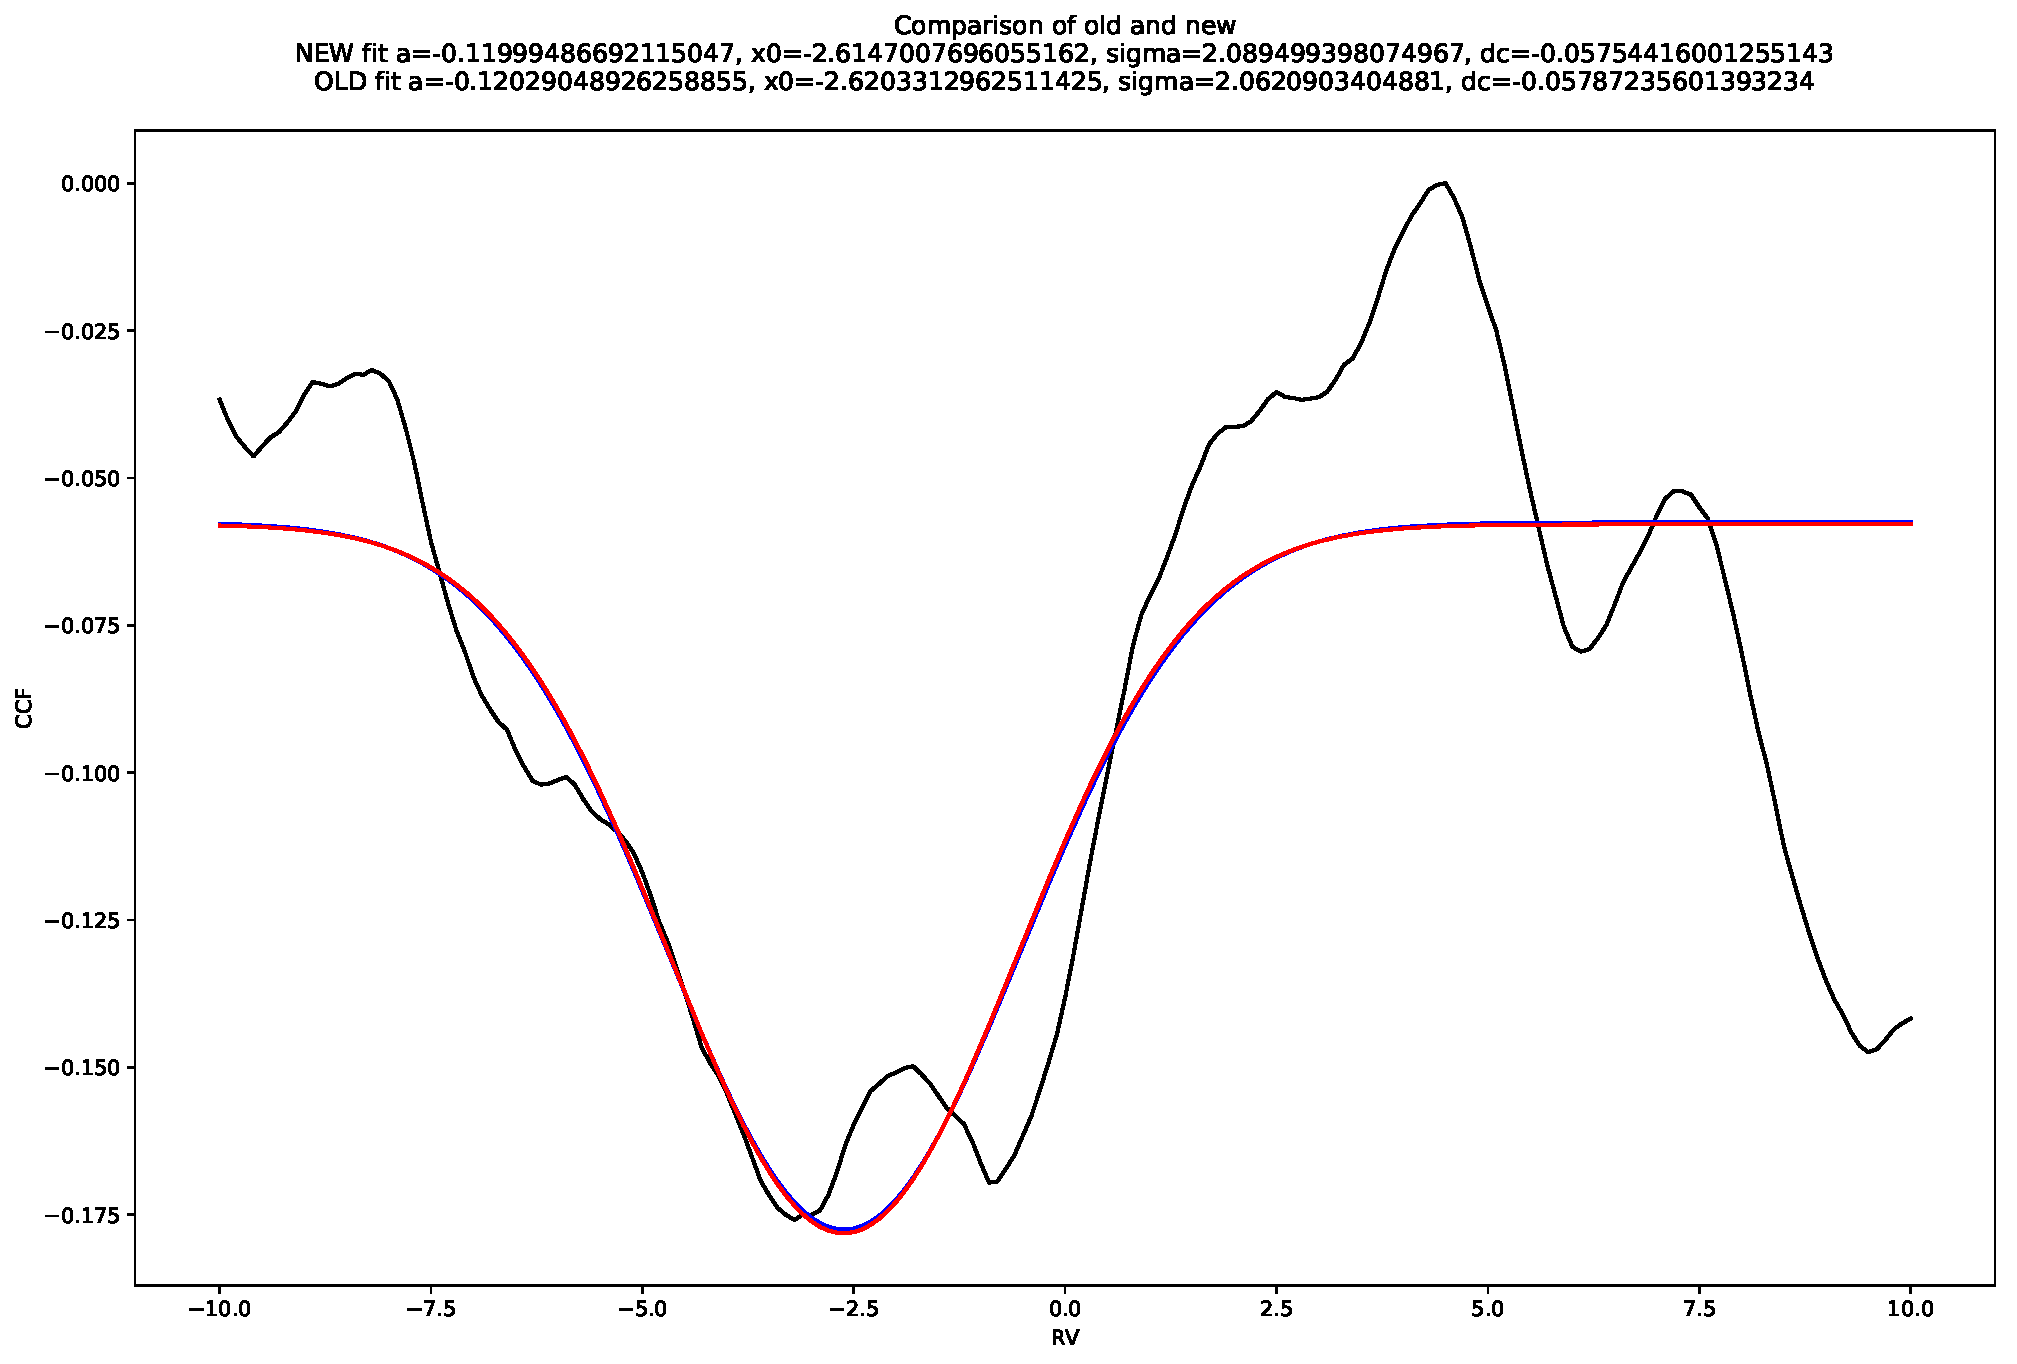
\includegraphics[width=.8\textwidth]{Figures/CCF_fitting_difference.pdf}
\end{center}
\caption{ The difference between the CCF fits from FORTRAN and python. `old' here signifies the AT4-V48 DRS code, `new' the python 3 implementation. `a' here is the amplitude of the Gaussian, `x0' is the Gaussian center, `sigma' is the full-width half-maximum of the Gaussian and `dc' is the continuum level. \label{figure:ccf_fitting_probelm}}
\end{figure}

\clearpage
\begin{landscape}
\begin{tabular}{lcccccc}
\hline
name & Time py3 [s] & Time py2 [s] & Time AT4-V48 [s] & AT4/py3 & AT4/py2 & py3/py2 \\
\hline
\hline
\calDARK & 1.89 & 1.84 & 4.66 & 2.46 & 2.53 & 1.03 \\
\calbadpix & 1.55 & 1.4 & 2.88 & 1.86 & 2.07 & 1.11 \\
\callocRAW {\hskip 0pt}(flat\_dark) & 3.23 & 3.01 & 7.37 & 2.28 & 2.44 & 1.07 \\
\callocRAW {\hskip 0pt}(dark\_flat) & 2.21 & 2.02 & 6.0 & 2.72 & 2.97 & 1.09 \\
\calSLIT & 4.39 & 4.41 & 9.36 & 2.13 & 2.12 & 0.99 \\
\calFFraw {\hskip 0pt}(flat\_dark) & 4.58 & 3.67 & 25.0 & 5.46 & 6.81 & 1.25 \\
\calFFraw {\hskip 0pt}(dark\_flat) & 4.14 & 3.47 & 23.42 & 5.66 & 6.75 & 1.19 \\
\calextractRAW {\hskip 0pt}(fp\_fp02a203.fits AB A B C) & 13.75 & 12.92 & 90.83 & 6.61 & 7.03 & 1.06 \\
\calextractRAW {\hskip 0pt}(fp\_fp03a203.fits AB A B C) & 13.46 & 12.57 & 92.25 & 6.85 & 7.34 & 1.07 \\
\calextractRAW {\hskip 0pt}(fp\_fp04a203.fits AB A B C) & 13.43 & 12.97 & 88.04 & 6.56 & 6.79 & 1.04 \\
\calDRIFTRAW & 7.29 & 6.88 & 0.49 & 0.07 & 0.07 & 1.06 \\
\calDRIFTE & 1.32 & 1.3 & 3.07 & 2.33 & 2.36 & 1.01 \\
\calDRIFTPEAK & 12.4 & 12.21 & 15.15 & 1.22 & 1.24 & 1.02 \\
\calCCF & 2.52 & 2.53 & 1.57 & 0.63 & 0.62 & 0.99 \\
\hline
Total & 86.16 & 81.21 & 370.09 & 4.3 & 4.56 & 1.06 \\
\hline
\hline
\end{tabular}
\captionof{table}{Table showing the timings of the python 3, python 2 and AT4-V48 tests. Computed are the speed up ratios between the various tests. \label{table:speed_tests}}
\end{landscape}



\clearpage
\begin{landscape}
{\footnotesize
\begin{tabular}{lllllllr}
\hline
\hline
  \multicolumn{1}{c}{Recipe} &
  \multicolumn{1}{c}{Type} &
  \multicolumn{1}{c}{Difference} &
  \multicolumn{1}{c}{Mean} &
  \multicolumn{1}{c}{Median} &
  \multicolumn{1}{c}{StDev} &
  \multicolumn{1}{c}{$log_{10}$(Diff)} &
  \multicolumn{1}{c}{Note} \\
\hline

& & & & & \\

\calbadpix & DATA & Difference image is non-zero &  &  &  & -0.975035 & 1 \\
\calbadpix & DATA & axis=0 (mean,median,std) & 0.246589 & 0.0 & 0.431025 & -0.975035  & 1 \\
\calbadpix & DATA & axis=1 (mean,median,std) & 0.248678 & 0.0 & 0.432247 & -0.975035  & 1 \\
\calbadpix & DATA & diff (mean,median,std) & -0.002088 & 0.0 & 0.045652 & -0.975035  & 1 \\

& & & & & \\

\hline
  \multicolumn{1}{c}{Recipe} &
  \multicolumn{1}{c}{Type} &
  \multicolumn{1}{c}{Difference} &
  \multicolumn{1}{c}{Old value} &
  \multicolumn{1}{c}{New value} &
  \multicolumn{1}{c}{difference} &
  \multicolumn{1}{c}{$log_{10}{Diff}$} &
  \multicolumn{1}{c}{Note} \\
 \hline

& & & & & \\

\callocRAW (flat\_dark) & HEADER & key=VERSION old,new,diff & SPIROU\_ & SPIROU\_0.0.057 &  &  & 2 \\
\callocRAW (flat\_dark) & HEADER & key=VERSION old,new,diff & SPIROU\_ & SPIROU\_0.0.057 &  &  & 2 \\
\callocRAW (dark\_flat) & HEADER & key=VERSION old,new,diff & SPIROU\_ & SPIROU\_0.0.057 &  &  & 2 \\
\callocRAW (dark\_flat) & HEADER & key=VERSION old,new,diff & SPIROU\_ & SPIROU\_0.0.057 &  &  & 2 \\
\calSLIT & HEADER & key=VERSION old,new,diff & SPIROU\_ & SPIROU\_0.0.057 &  &  & 2 \\
\calFFraw (flat\_dark) & HEADER & key=VERSION old,new,diff & SPIROU\_ & SPIROU\_0.0.057 &  &  & 2 \\
\calFFraw (flat\_dark) & HEADER & key=VERSION old,new,diff & SPIROU\_ & SPIROU\_0.0.057 &  &  & 2 \\
\calFFraw (dark\_flat) & HEADER & key=VERSION old,new,diff & SPIROU\_ & SPIROU\_0.0.057 &  &  & 2 \\
\calFFraw (dark\_flat) & HEADER & key=VERSION old,new,diff & SPIROU\_ & SPIROU\_0.0.057 &  &  & 2 \\
\callocRAW (flat\_dark) & HEADER & key=QC old,new,diff & PASSED & 1 &  &  & 3 \\
\callocRAW (flat\_dark) & HEADER & key=QC old,new,diff & PASSED & 1 &  &  & 3 \\
\callocRAW (dark\_flat) & HEADER & key=QC old,new,diff & PASSED & 1 &  &  & 3 \\
\callocRAW (dark\_flat) & HEADER & key=QC old,new,diff & PASSED & 1 &  &  & 3 \\
\calbadpix & HEADER & key=BBAD old,new,diff & 24.658989 & 24.867844 & -0.20885 & -2.072131  & 1 \\
\calbadpix & HEADER & key=BBFLAT old,new,diff & 1.317787 & 1.6633749 & -0.345587 & -0.581287  & 1 \\
\calCCF & HEADER & key=CCFCONTR old,new,diff & 2.844530 & 2.835287 & 0.009243 & -2.486784 & 4 \\
\calCCF & HEADER & key=CCFFWHM old,new,diff & 4.346651 & 4.261318 & 0.08533 & -1.698425 & 4 \\
\calCCF & HEADER & key=CCFMACPP old,new,diff & 422345 & 422345.043882 & -0.043882 & -6.983377 & 4 \\
\calCCF & HEADER & key=CCFRV old,new,diff & -0.547685 & -0.553049 & 0.005365 & -2.009001 & 4 \\
\calCCF & HEADER & key=CCFRVC old,new,diff & -0.547685 & -0.553049 & 0.005365 & -2.009001 & 4 \\

& & & & & \\

\hline
\hline
\end{tabular}
\captionof{table}{Table showing all image and header outputs that failed the $log_{10}$(Difference) test between the `old' (AT4-V48) and `new' (python 2/python 3) versions. \label{table:failed_tests}}
}
\begin{enumerate}
\item Explained by the difference in using 90th percentile and sorting to select 90th index
\item Explained by an error in old code: \definevariable{text:drs_version}{DRS\_VERSION} not passed to header
\item Explained by an error in old code: \definevariable{ch:variables:qualitycontrol}{QC} not passed to header
\item Explained by the difference in using \Program{fitgaus} (FORTRAN) and \Program{scipy.curve\_fit} (python) functions.
\end{enumerate}
\end{landscape}


